\documentclass[a4paper,12pt]{article}


%%%%%%%%%%%%%%%%%%%%%%%%%%%%%%%%%%%%%%%%%%%%%%%%%%%%%%%%%%%%
% DELIVERABLE META DATA
%
% Modify so that the meta data is correct for this deliverable.
%%%%%%%%%%%%%%%%%%%%%%%%%%%%%%%%%%%%%%%%%%%%%%%%%%%%%%%%%%%%

% The WP to which the deliverable belongs (the x in Dx.y).

\def\nlafetMajor{2}

% The deliverable number within the WP (the y in Dx.y).

\def\nlafetMinor{1}

% A long title for the deliverable (for the front page).
%
% Look up the correct title in the grant agreement.

\def\nlafetTitle{One-sided Matrix Factorizations}

% A short title for the deliverable (for the header).
%
% Shorten the title if necessary to fit the header.

\def\nlafetShortTitle{One-sided Matrix Factorizations}

% The month when this version was published.

\def\nlafetMonth{April}

% The year when this version was published.

\def\nlafetYear{2017}

% The scheduled delivery of this deliverable.
%
% This is the last day of the delivery month found in the grant
% agreement. November 2015 is referred to as M1. For example, if the
% delivery month is M6, then the date below should read 2016-04-30
% since April 2016 is M6.

\def\nlafetScheduledDelivery{2017-04-31}

% The actual delivery of this deliverable.
%
% This is the date the deliverable was actually delivered. Do not
% change this field until the actual delivery.

\def\nlafetActualDelivery{(not yet delivered)}

% The current major and minor version number of this document.
%
% The bigger the number, the newer the version. How you assign major
% and minor version numbers is up to you. The sole purpose of the
% version number is to make it easier to reference different versions.

\def\nlafetVersionMajor{0}
\def\nlafetVersionMinor{1}

% The short name (UMU/UNIMAN/STFC/INRIA) of the partner responsible
% for this deliverable.

\def\nlafetResponsiblePartner{UNIMAN}

% The dissemination level.
%
% Either public or confidential. Look up the correct level in the the
% grant agreement.

% \def\nlafetDisseminationLevel{PU --- Public}
\def\nlafetDisseminationLevel{CO --- Confidential}






%%%%%%%%%%%%%%%%%%%%%%%%%%%%%%%%%%%%%%%%%%%%%%%%%%%%%%%%%%%%
% PACKAGES REQUIRED BY TEMPLATE
%
% Do not touch!
%%%%%%%%%%%%%%%%%%%%%%%%%%%%%%%%%%%%%%%%%%%%%%%%%%%%%%%%%%%%

% Input and font encoding.
\usepackage[utf8]{inputenc}
\usepackage[T1]{fontenc}
\usepackage{lmodern}

% Colored table.
\usepackage{xcolor}
\usepackage{colortbl}

% Graphics.
\usepackage{graphicx}

% Header/footer.
\usepackage{fancyhdr}

% Margins.
\usepackage[margin=25mm]{geometry}

% Total page count.
\usepackage{lastpage}

% URL typesetting.
\usepackage{url}

% Table with word wrap.
\usepackage{tabularx}


\usepackage{amsmath,amssymb}

\usepackage{subcaption}



%%%%%%%%%%%%%%%%%%%%%%%%%%%%%%%%%%%%%%%%%%%%%%%%%%%%%%%%%%%%
% HEADER / FOOTER
%
% Do not touch!
%%%%%%%%%%%%%%%%%%%%%%%%%%%%%%%%%%%%%%%%%%%%%%%%%%%%%%%%%%%%

\pagestyle{fancy}
\renewcommand{\footrulewidth}{\headrulewidth}
\lhead{\bf NLAFET}
\rhead{\bf D\nlafetMajor.\nlafetMinor: \nlafetShortTitle}
\lfoot{\url{http://www.nlafet.eu/}}
\cfoot{}
\rfoot{\thepage/\pageref{LastPage}}





%%%%%%%%%%%%%%%%%%%%%%%%%%%%%%%%%%%%%%%%%%%%%%%%%%%%%%%%%%%%
% TITLE PAGE
%
% Do not touch!
%%%%%%%%%%%%%%%%%%%%%%%%%%%%%%%%%%%%%%%%%%%%%%%%%%%%%%%%%%%%

\begin{document}

\begin{titlepage}
  \centering
  {
    
\includegraphics[width=0.8\textwidth]{NLAFET-logo2}
  }
  \par
  \vspace{5mm}
  {
    H2020--FETHPC--2014: GA 671633
  }
  \par
  \vspace{4cm}
  {
    \Huge
    D\nlafetMajor.\nlafetMinor\\[1em]
    \nlafetTitle
  }
  \par
  \vfill
  {
    \Large
    \nlafetMonth{}
    \nlafetYear
  }
\end{titlepage}



%%%%%%%%%%%%%%%%%%%%%%%%%%%%%%%%%%%%%%%%%%%%%%%%%%%%%%%%%%%%
% DOCUMENT INFORMATION
%
% Touch only the following sections:
% 1. REVISION HISTORY: Add rows as appropriate (remove the current
%    line first).
% 2. AUTHOR(S): List the authors and their organization.
% 3. INTERNAL REVIEWERS: List the internal reviewers and their organizations.
% 4. CONTRIBUTORS: List any additional contributors and their
%    organizations, or remove the section if there are no additional
%    contributors.
%%%%%%%%%%%%%%%%%%%%%%%%%%%%%%%%%%%%%%%%%%%%%%%%%%%%%%%%%%%%

\newpage




\noindent
\textsc{Document information}\\[1em]
\begin{tabular}{@{}ll}
  Scheduled delivery & \nlafetScheduledDelivery \\
  Actual delivery & \nlafetActualDelivery \\
  Version & \nlafetVersionMajor.\nlafetVersionMinor \\
  Responsible partner & \nlafetResponsiblePartner \\
\end{tabular}

\vspace{2em}




\noindent
\textsc{Dissemination level}\\[1em]
\nlafetDisseminationLevel

\vspace{2em}




% TODO: List the revision history.
\noindent
\textsc{Revision history}\\[1em]
\begin{tabularx}{\linewidth}{@{}|l|l|l|l|X|}
  \hline
  \rowcolor{orange}
  \bf Date & \bf Editor & \bf Status & \bf Ver. & \bf Changes \\
  \hline
  2017-04-11 & Samuel Relton & Final & 1.0 & Incorporated reviewer suggestions.\\
  2017-03-27 & Samuel Relton & Draft & 0.1 & Initial version of
                                             document produced. \\
  \hline
\end{tabularx}

\vspace{2em}




% TODO: List the authors.
\noindent
\textsc{Author(s)}\\[1em]
% First Last (UMU/UNIMAN/STFC/INRIA)
Negin Bagherpour (UNIMAN)\\
Samuel Relton (UNIMAN)\\
Mawussi Zounon (UNIMAN)

\vspace{2em}

% TODO: List the internal reviewers.
\noindent
\textsc{Internal reviewers}\\[1em]
Mirko Myllykoski (UMU)\\
Nicholas Higham (UNIMAN)\\
Vedran Novakovi\'{c} (STFC)

\vspace{2em}


% TODO: List additional contributors, if any.
\noindent
\textsc{Contributors}\\[1em]

\vspace{2em}





\noindent
\textsc{Copyright}\\[1em]
This work is \copyright by the NLAFET Consortium, 2015--2018.
Its duplication is allowed only for personal, educational, or research uses.

\vspace{2em}





\noindent
\textsc{Acknowledgements}\\[1em]
This project has received funding from the \emph{European Union's Horizon 2020 research and innovation programme} under the grant agreement number 671633.





%%%%%%%%%%%%%%%%%%%%%%%%%%%%%%%%%%%%%%%%%%%%%%%%%%%%%%%%%%%%
% TABLES OF CONTENTS
%
% Remove list of figures/tables if not applicable.
%%%%%%%%%%%%%%%%%%%%%%%%%%%%%%%%%%%%%%%%%%%%%%%%%%%%%%%%%%%%

\newpage

\renewcommand{\contentsname}{Table of Contents}
\tableofcontents

% TODO: Remove if there are no figures.
\listoffigures

% TODO: Remove if there are no tables.
\listoftables





\newpage

%%%%%%%%%%%%%%%%%%%%%%%%%%%%%%%%%%%%%%%%%%%%%%%%%%%%%%%%%%%%
% START OF THE ACTUAL DELIVERABLE
%
% The content below acts merely as a placeholder. Use whatever
% disposition is most appropriate.
%%%%%%%%%%%%%%%%%%%%%%%%%%%%%%%%%%%%%%%%%%%%%%%%%%%%%%%%%%%%

%%%%%%%%%%%%%%%%%%%%%%%%%%%%%%
\section{Introduction}
\label{sec.introduction}
%%%%%%%%%%%%%%%%%%%%%%%%%%%%%%
The primary use of high-performance linear algebra software
in scientific applications is in solving linear systems.
Whether one needs to solve a system arising from the discretization of
a partial differential equation,
fit a model to some data in a least-squares sense,
or solve a KKT system in an optimization problem,
there will undoubtedly be linear systems to solve.
As applications have evolved these systems have become larger,
necessitating the use of high-performance linear algebra routines
to solve them in a reasonable amount of time.
Usually such dense systems are solved using
the Cholesky, $LU$, $QR$, or symmetric-indefinite factorizations
(collectively known as the one-sided factorizations).
The LAPACK names for these factorizations are
POTRF, GETRF, GEQRF, and (SY/HE)TRF, respectively.

In this work we compare different implementations of
these routines using the novel task-based programming paradigm.
Whilst this has existed for a number of years in the runtimes
described in section~\ref{sec.runtime_systems},
it has only recently been supported in OpenMP, since version~4.0.
Our efforts in applying OpenMP to this problem
are collated in the new release of the PLASMA library~\cite{addh09}
which aims to implement the entire of the LAPACK standard~\cite{lug99}
in this fashion.

The task-based programming paradigm breaks each linear algebra
problem into a series of tasks operating on blocks of data.
These tasks can depend on one another:
for instance in a typical panel factorization algorithm
the tasks used to factorize the panel need to be completed
before the tasks to update the trailing matrix can begin.
Typically these interdependencies are expressed using a
directed acylic graph (DAG),
which is also known as a task-graph.
The nodes of the graph are functions to be computed and
the edges denote dependencies between the output of one task
to the input of another.
As an example,
the DAG for a small Cholesky factorization is shown in
Figure~\ref{fig.chol_dag} below.
\begin{figure}[th]
  \centering
  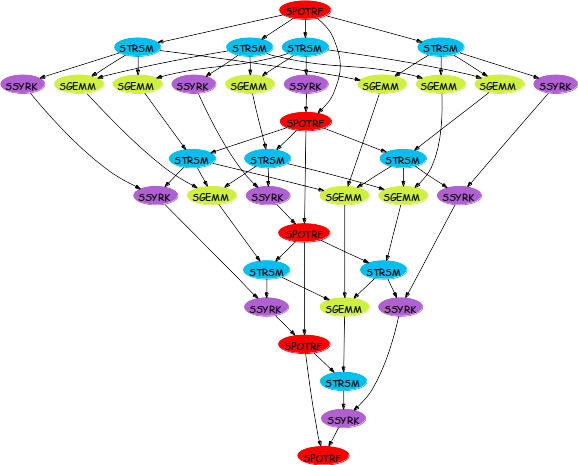
\includegraphics[scale=.6]{fig/spotrf_dag.png}
  \caption{DAG for a small Cholesky factorization.}
  \label{fig.chol_dag}
\end{figure}

The red, blue, purple, and green tasks correspond to
SPOTRF, STRSM, SSYRK, and SGEMM tasks
whilst the arrows show the dependency between tasks.
Each task will (usually) be performed by a single core
and each completed task leads to further tasks becoming available.
Once the dependencies for a task have been fulfilled it
can immediately be assigned to a core.
Some more detail on this model of programming
used in a linear algebra context is given in section~\ref{sec.tile}.

The goal of this report is to compare implementations of
the four factorizations mentioned above
using a variety of runtime systems in a multi-core environment.
Each system is utilizing the same DAG and differs only in the way
that tasks are assigned to the available cores.
We also compare against reference Intel MKL
for completeness.
The performance of each implementation is measured
on modern computer architectures:
an Intel Broadwell NUMA node
and the Intel Xeon Phi (codenamed Knights Landing).

The rest of this document is arranged as follows.
Section~\ref{sec.tile} gives an introduction
to the use of tile-based algorithms and
task-based programming in linear algebra.
In section~\ref{sec.runtime_systems} we give a
brief summary of the capabilities of the various
runtime systems used to implement the four factorizations.
Section~\ref{sec.arch} gives more detail on the
software libraries and architectures used in our experiments.
Sections~\ref{sec.cholesky}--\ref{sec.ldlt} then
contain the experimental results for the four
one-sided factorizations.
Finally we summarize the results and give some conclusions
in section~\ref{sec.conclusions}.

%%%%%%%%%%%%%%%%%%%%%%%%%%%%%%
\section{Tile-based one-sided factorization}
\label{sec.tile}
While LAPACK~\cite{lug99} linear algebra factorization
algorithms were successful in exploiting early cache-based
architectures, they have shown significant performance
limitations on modern many/multi-core architectures and many
well-tuned LAPACK-style kernels
fail to achieve satisfactory performance on these
architectures~\cite{agullo2009comparative}.
As reported by Dongarra et al\@.~in~\cite{dongarra2011achieving},
three factors contribute to this
performance penalty.

The first factor is the fork-join parallelism
model appearing in LAPACK when it is linked with multi-threaded BLAS.
This model induces a high overhead on
massively parallel architectures since it introduces many unnecessary
synchronization points, keeping many computational resources frequently
idle.
Secondly, LAPACK processes data at a coarse granularity,
typically working on the block-column level (also known as a panel),
which fails to exhibit enough parallelism to
keep all the cores busy.
Finally, while all factorization algorithms in LAPACK are based on
a recursive panel factorization followed by an update to the
corresponding trailing matrix,
the panel factorization uses memory-bound operations
(i.e.\ level-1 and level-2 BLAS operations).

In order to use modern many/multi-core architectures at full
efficiency, a new generation of linear algebra libraries such as
PLASMA~\cite{DBLP:journals/corr/abs-0709-1272} and FLAME~\cite{FLAWN3}
\textcolor{red}{CHANGE FLAME REF, THEY DIDN'T DO THIS IN 2001!}
have cast LAPACK panel-based algorithms into tile algorithms. Tile
algorithms enjoy the property of addressing each of the three
drawbacks that keep LAPACK from providing a reasonable performance on
modern massively parallel architectures.
In fact, tile algorithms operate at a
finer granularity by dividing the whole matrix into
small square tiles which are more likely to fit into fast memory,
such as the L2 cache of a CPU, as illustrated in Figure~\ref{fig:tile_algo}.
\begin{figure}[th]
  \captionsetup[subfigure]{justification=justified,singlelinecheck=false}
  \begin{subfigure}[t]{0.3 \textwidth}
    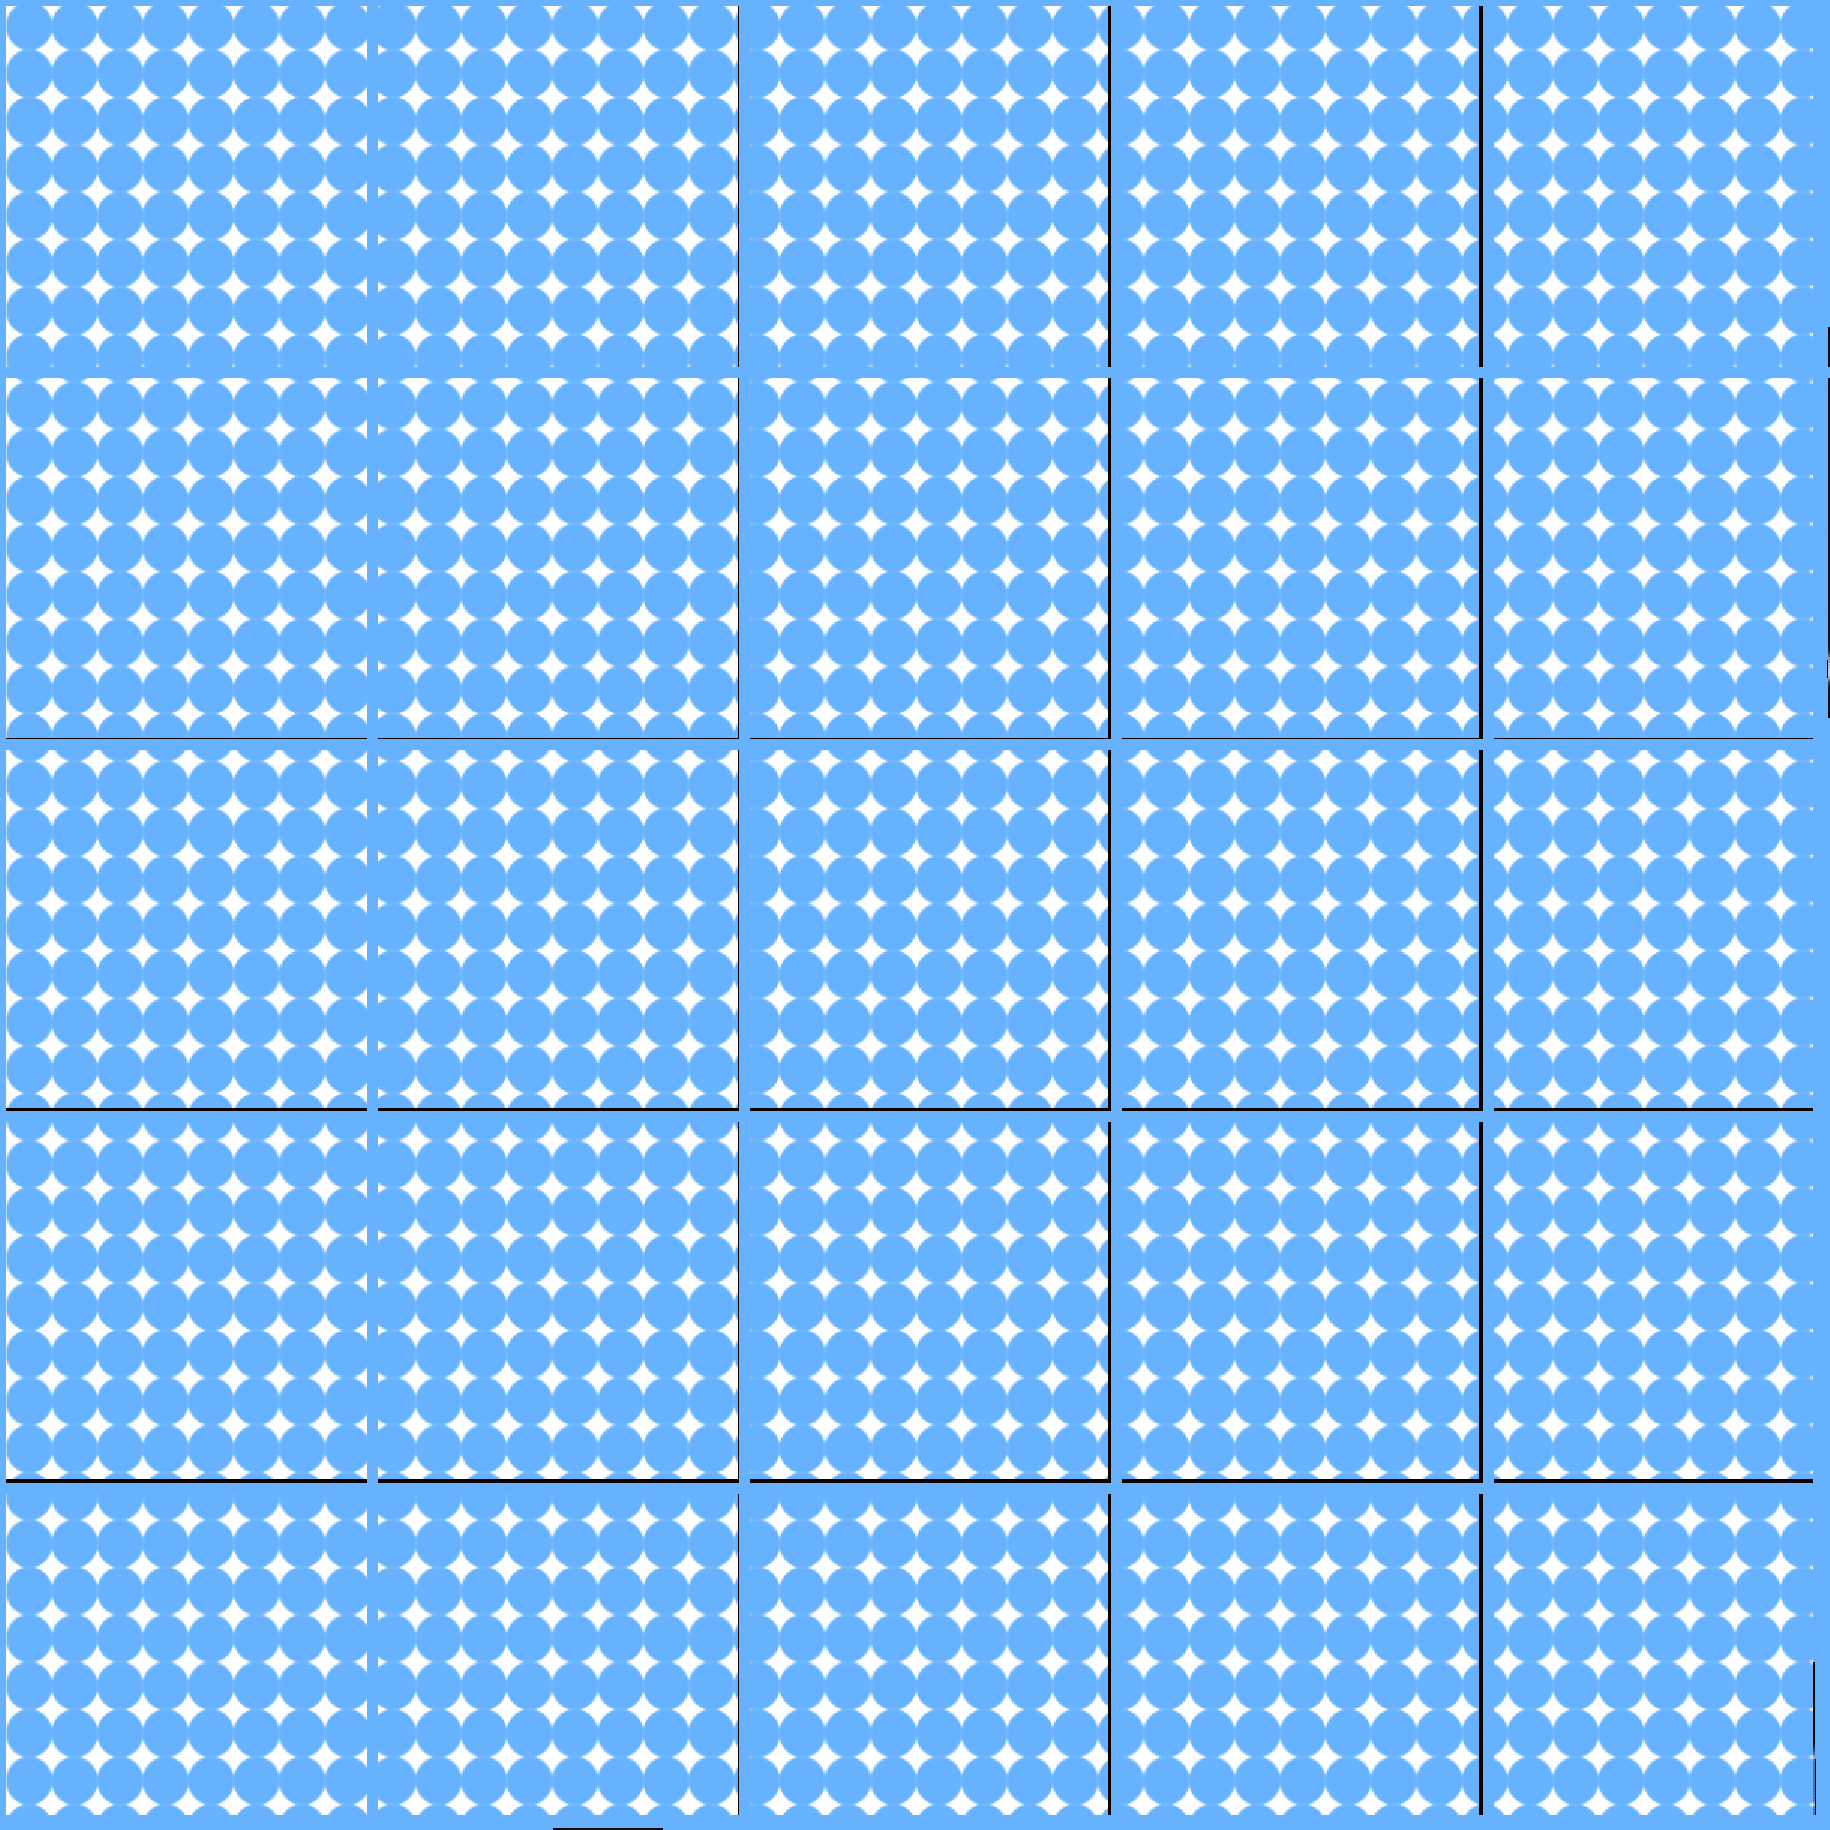
\includegraphics[width=3.5cm, height=3.5cm]{fig/one-sided-initial}
    \caption{\label{fig:initial_matrix}Initial matrix.}
  \end{subfigure}
  \hfill
  \begin{subfigure}[t]{0.3 \textwidth}
    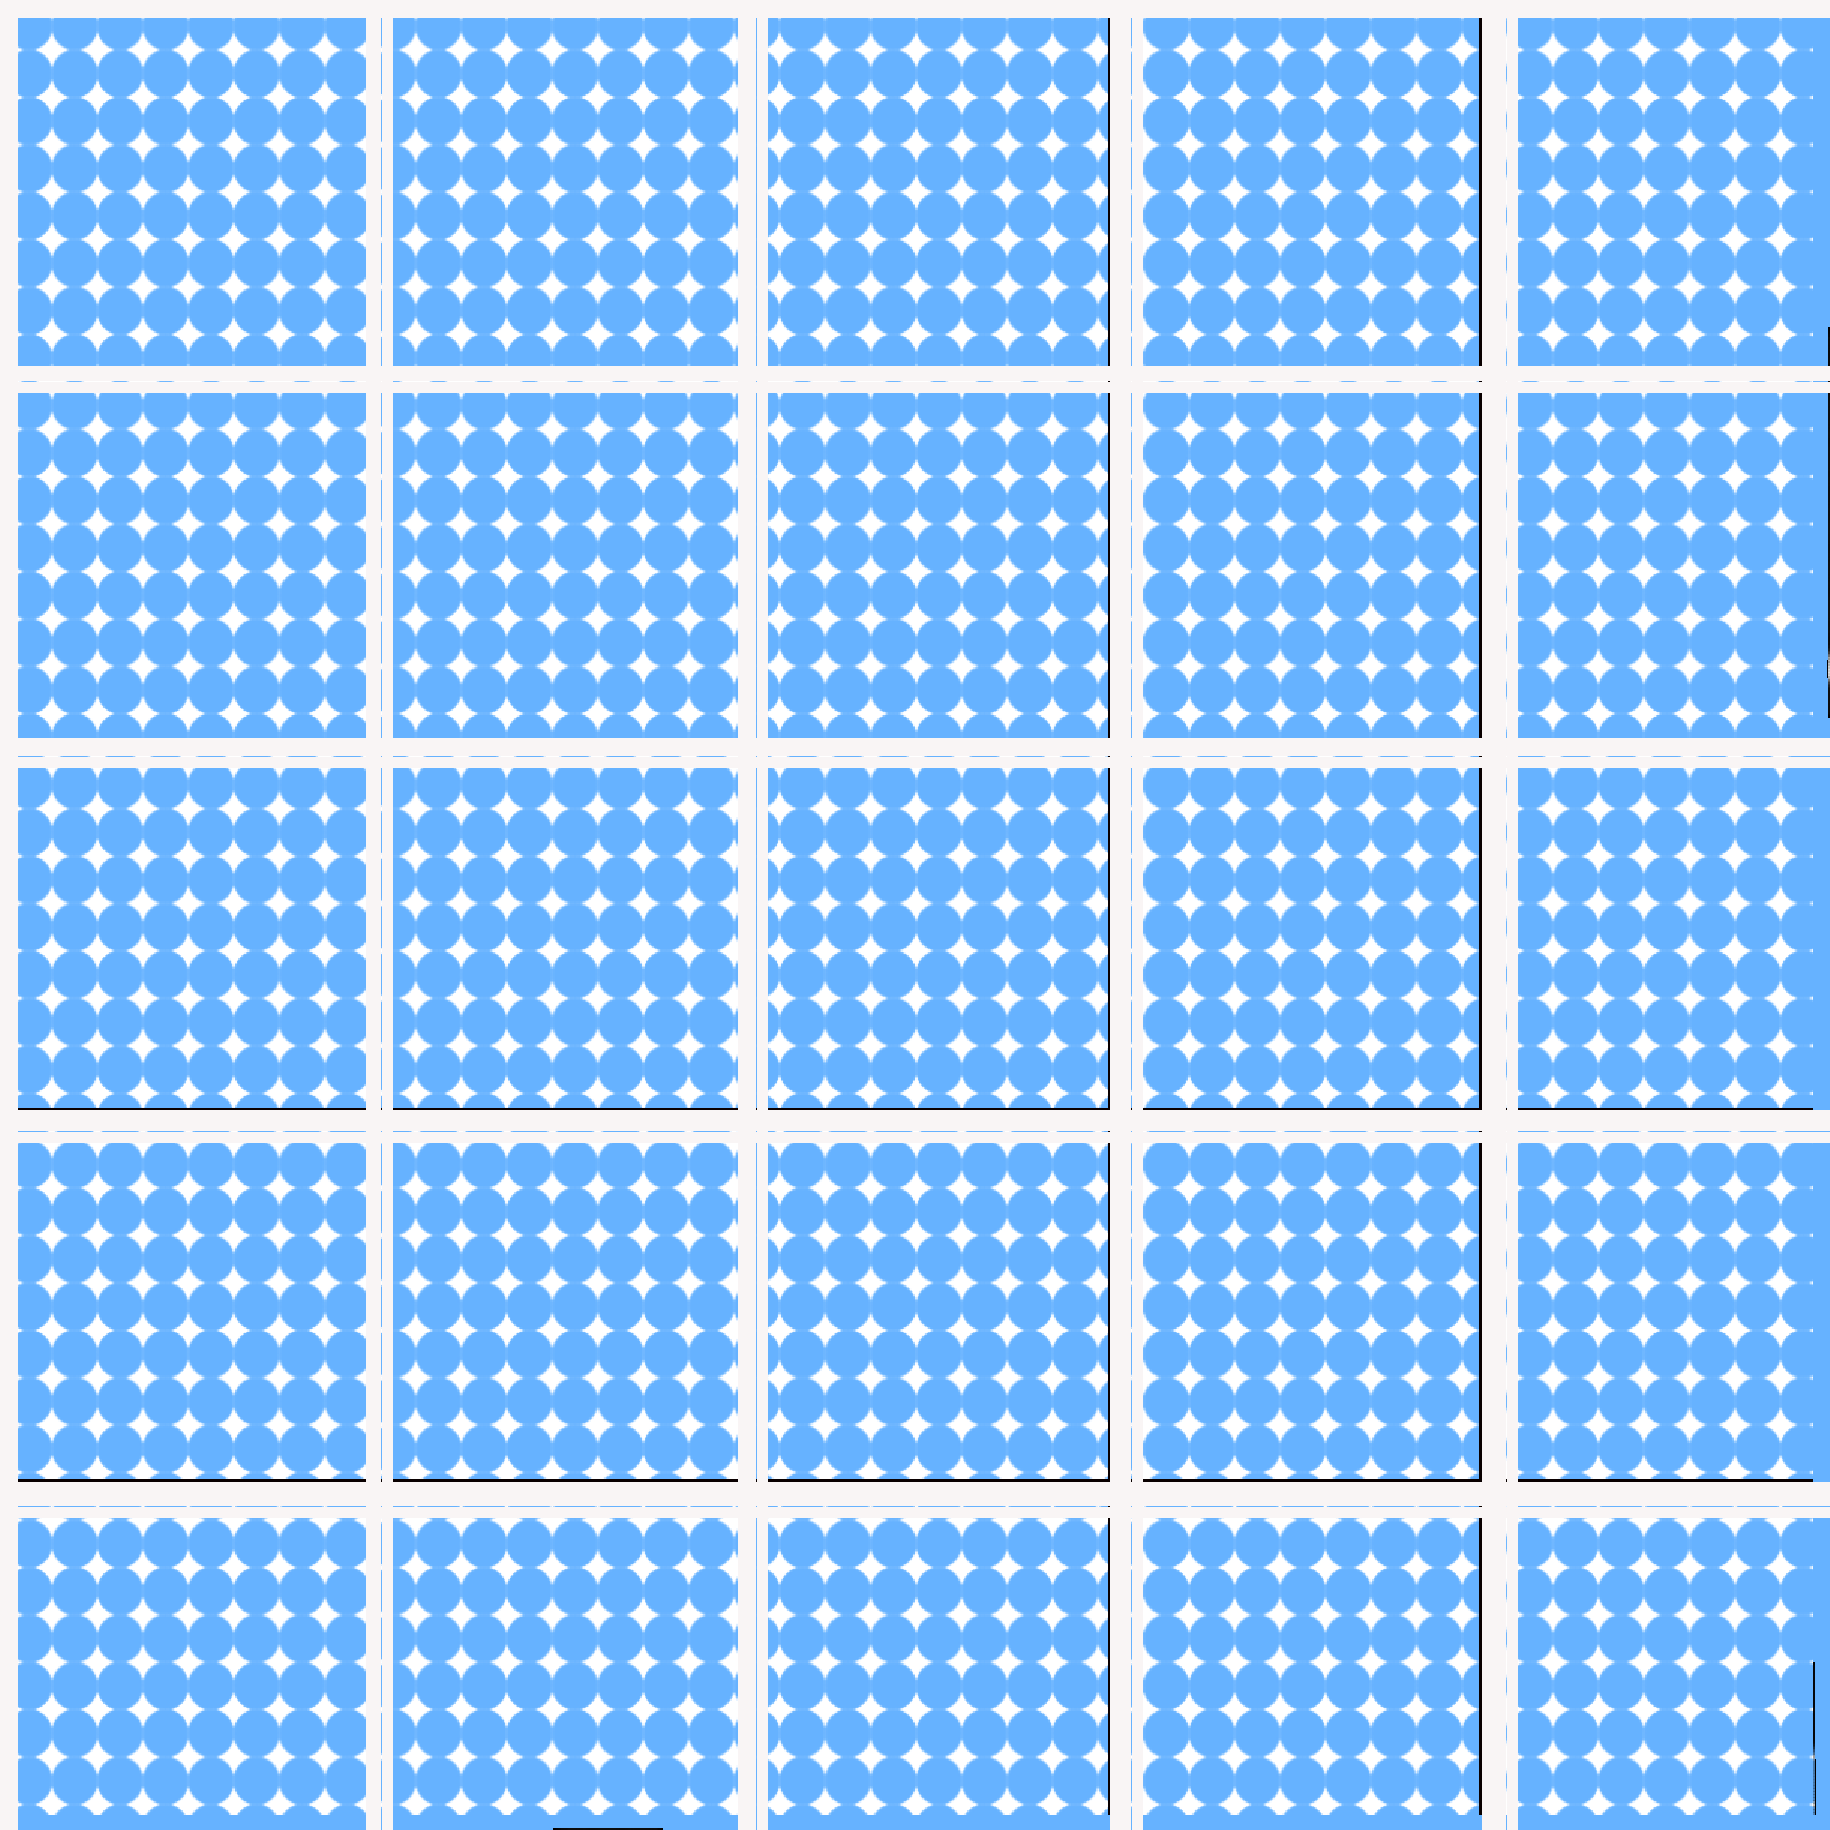
\includegraphics[width=3.5cm, height=3.5cm]{fig/one-sided-tile}
    \caption{\label{fig:tile_matrix}
      $5\times 5$ tile matrix.}
  \end{subfigure}
  \hfill
    \begin{subfigure}[t]{0.3 \textwidth}
    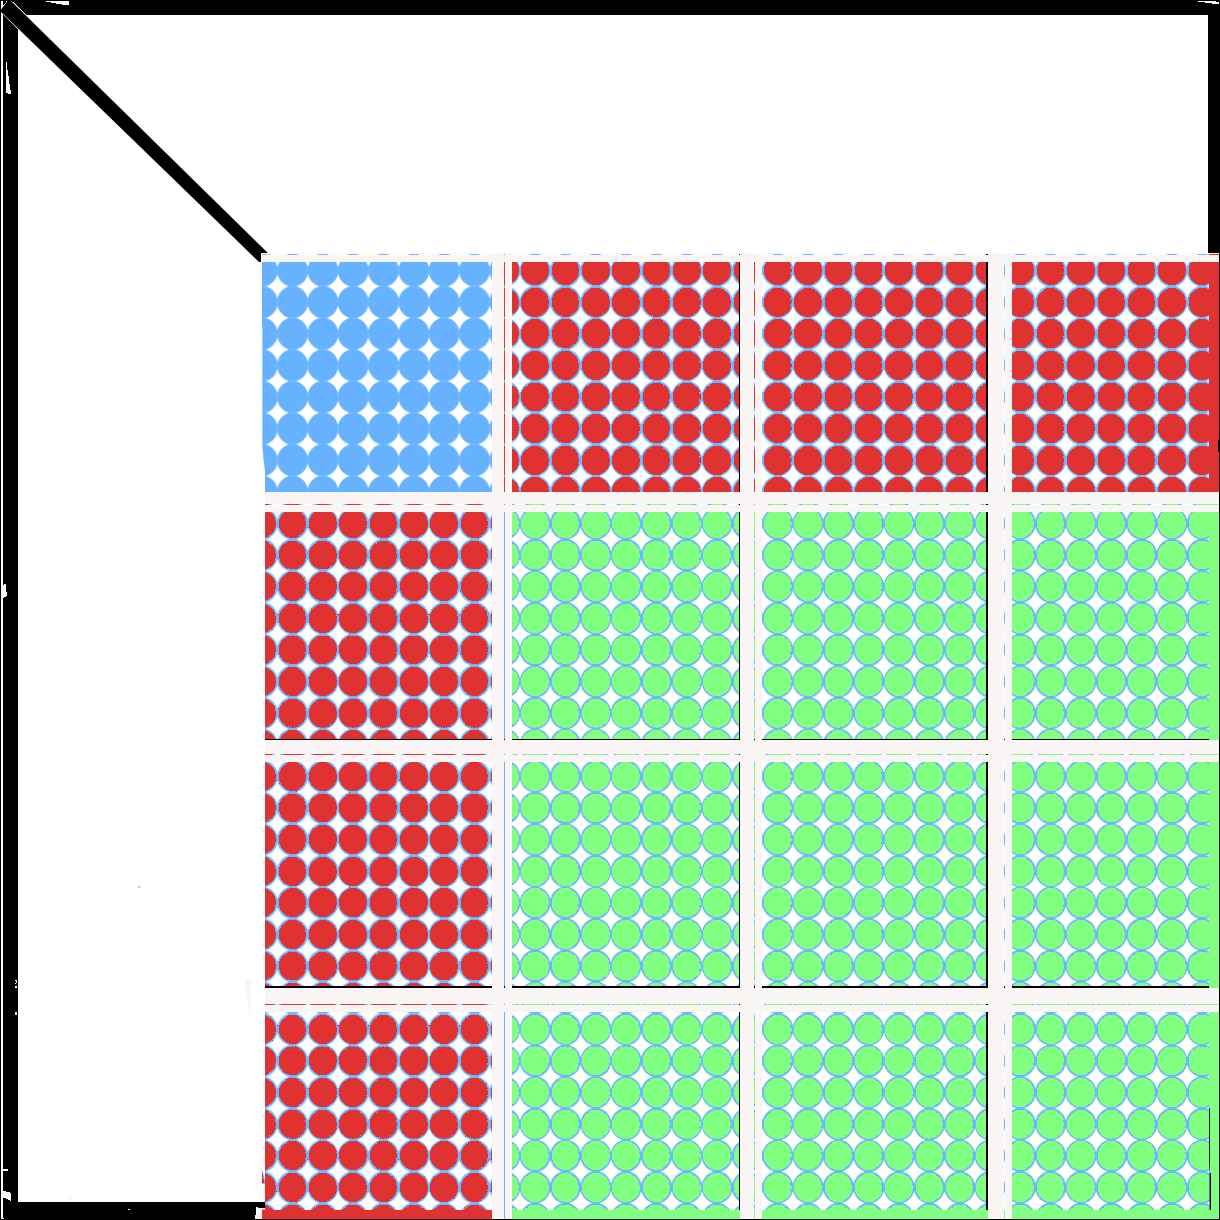
\includegraphics[width=3.5cm, height=3.5cm]{fig/one-sided-tile-facto}
    \caption{\label{fig:tile_facto}
     Many kernels operating on different tiles in parallel.}
  \end{subfigure}
  \caption{Illustration of matrix division in square tiles as is the case
    in tile algorithms. This helps working at  a finer granularity to
    keep the maximum number of cores busy.}
    \label{fig:tile_algo}
\end{figure}

The order of execution of the tasks in tile algorithms are commonly
represented in the form of a DAG in which each node represents a task, while
the edges represent the data dependencies between the tasks.  These
tasks are then scheduled by a runtime system that checks the
dependencies and takes care of launching tasks on appropriate cores.

The superiority of the tile layout algorithms over traditional
approaches has been demonstrated conclusively through a one-sided
factorization benchmark suite~\cite{agullo2009comparative}.

In the last few years,
the PLASMA development team dedicated their full
energy to designing highly efficient tile
algorithms for one-sided factorizations.
In 2008, Buttari et al.~\cite{buttari2008parallel},
introduced the first algorithm for parallel tiled $QR$ factorization for
multicore architectures.
This algorithm was extended in 2010 by
Hadri et al.~\cite{hadri2010tile} to present a new fully asynchronous
method for computing a $QR$ factorization of tall and skinny matrices.
The Cholesky and $LU$ factorization versions are studied
in~\cite{DBLP:journals/corr/abs-0709-1272}, while the algorithm to
compute the $LDL^T$ factorization of symmetric indefinite matrices is
discussed in~\cite{becker2011towards}
(though we add pivoting in the implementations compared here).

This work revisits the state-of-the-art tile algorithms for
one-sided factorizations and provides an
efficient task-based OpenMP implementation for comparison with
other runtime systems.

%%%%%%%%%%%%%%%%%%%%%%%%%%%%%%



%%%%%%%%%%%%%%%%%%%%%%%%%%%%%%
\section{Runtime systems}
\label{sec.runtime_systems}
%%%%%%%%%%%%%%%%%%%%%%%%%%%%%%
Each runtime system used in this report has a variety of
features that makes them unique.
In this section we will describe the unique features of each runtime
system that we compare.
Even though this report focuses on multi-core environments,
some of the runtime systems also support the use of accelerators
and can scale to distributed architectures with
minimal effort.
The runtime systems that we will use are
\begin{itemize}
\item OpenMP\footnote{\url{http://www.openmp.org}},
\item Quark, and
\item StarPU.
\end{itemize}

OpenMP is the standard way to parallelize code over a
multi-core architecture.  The pragma
\texttt{\#pragma omp parallel for}
is a well-known method for parallelizing loops
over the available cores.
However, it is only recently that OpenMP
began to support task-based programming.  This is the main drawback of
using task-based OpenMP currently: advanced features, such as
assigning a priority to critical tasks or choosing from a variety of
different task scheduling strategies, are either not in the current
OpenMP standard or have not been widely implemented.  This is due to
the relative immaturity of task-based programming within OpenMP.
Meanwhile, the benefits to using OpenMP are its wide availability and
lightweight framework (meaning there are few significant overheads
when using the task-based paradigm).  As is well known, current
OpenMP implementations do not widely support the use of accelerators
and OpenMP is not designed for distributed memory computation.

Quark is a research project implementing task-based programming
produced by ICL at the University of Tennessee%
\footnote{More information available at
  \url{http://icl.utk.edu/quark/} as of 23rd March 2017.}.
It was one of the first frameworks to support this style
of programming and as such does not follow all of the standards
defined by the OpenMP Standardisation Committee.
Since Quark is a fairly old research project it is not under current
development:
at the moment it is still highly relevant but this will of course fade
in the coming years as OpenMP evolves.
Quark does not support accelerators or distributed memory.

StarPU is a runtime system built by Inria Bordeaux~\cite{starpu11}.
The system supports the use of both GPUs and
distributed memory computation,
though neither of these features are used in this report
to ensure a fair comparison.
Another key advantage of StarPU over the other runtime systems
is the incorporation of multiple different task scheduling strategies.
In this report we will use the ``eager'', ``dmda'', and ``ws''
strategies.

First,
in the ``eager'' strategy,
each core draws tasks independently from a centralised queue
whenever they become idle.
This strategy does not allow for data prefetching since the scheduling
decision is taken as late as possible.
Meanwhile, the ``dmda'' (deque model data aware) strategy
uses an estimate of the runtime
(and memory transfer time) of each task to schedule them into
multiple queues for each core,
aiming to minimize the overall runtime.
The downside to this strategy is the more complicated scheduling required,
which may lead to overheads in task scheduling;
these overheads would be insignificant on larger distributed computations
where data transfer times dominate,
though it remains to be seen how it performs on a single node.
Each run of the computation using the ``dmda'' strategy
gives the scheduling system more information
upon which to base its future decisions.
Finally,
the ``ws'' (work-stealing) strategy allows each core to
steal work from the other cores when they becomes idle.
This is designed to keep all cores busy at all times.

There are a number of other scheduling strategies implemented within
StarPU but these are the ones best-suited to
operation on a single node.
The downside to StarPU is the additional overhead in task scheduling
as a result of the numerous advanced features supported.
However,
the support for accelerators and distributed memory
means that StarPU is readily applicable to heterogeneous computing
environments.
We also make use of the KStar source-to-source compiler in this work,
which automatically converts OpenMP task-based programs to
StarPU programs%
\footnote{Downloaded from \url{http://kstar.gforge.inria.fr/#!index.md} on
  23rd March 2017.}.

There are also other runtime systems that could be considered,
in particular ParSec (also from ICL at the University of Tennessee)%
\footnote{Available from
  \url{https://bitbucket.org/icldistcomp/parsec} as of 23rd March 2017.}.
ParSec supports the use of accelerators and distributed memory machines,
but is currently rather difficult to use due to the
different way the DAG is described.
The ParSec team is currently working on a simplified interface,
similar to that used by StarPU,
along with a similar source-to-source compiler for converting OpenMP code.

%%%%%%%%%%%%%%%%%%%%%%%%%%%%%%
\section{Experimental setup}
\label{sec.arch}
%%%%%%%%%%%%%%%%%%%%%%%%%%%%%%

%%%%%%%%%%%%%%%%%%%%%%%%%%%%%%
\begin{table}[t]
  \centering
  \caption{Architecture details for the Intel Broadwell NUMA node and
    the Intel Xeon Phi (KNL).
    Note that gcc is used for compatibility with the KStar
    source-to-source compiler.}
  \vspace{.5em}
  \begin{tabular}{|r | l | l |}
    \hline
    \textbf{Platform} & Xeon E5-2690 v4 & Xeon Phi 7250\\
    \textbf{Cores}    & $2 \times 14$ (2.6GHz) & 68 (1.4GHz)\\
    \textbf{On-chip Memory} & L1 32KB (per core) & L1 32KB (per core)\\
                      & L2 256KB (per core) & L2 512KB (per core)\\
                      & L3 35MB (per NUMA island)  & MCDRAM 16GB\\
    \textbf{Main Memory} & 128GB DDR4 & 320GB DDR4\\
    \textbf{Bandwidth} & 76.8 GB/s & 115.2 GB/s\\
    \textbf{Compiler} & gcc 5.4.0 & gcc 6.1.0\\
    \textbf{MKL version} & 17.0.1 & 17.0.2\\
    \hline
  \end{tabular}
  \label{tab.arch}
\end{table}
%%%%%%%%%%%%%%%%%%%%%%%%%%%%%%

Each of our experiments covering the four one-sided factorizations
will be performed on two different architectures,
to show the level of performance that can be expected on
modern multi-core platforms.
In Table~\ref{tab.arch} we describe each architecture in more detail
and list the compilers and versions of MKL used but,
briefly, we have:
\begin{itemize}
\item a 2-socket NUMA node with Intel Broadwell processors, and
\item the new Intel Xeon Phi (codenamed Knights Landing, i\@.e\@.~KNL).
\end{itemize}
Note that, on the Intel KNL,
we are using the DDR4 memory as opposed to the MCDRAM.
Using the MCDRAM explicitly can result in much higher performance
rates,
but the amount of available memory is limited.

In each scenario we will compare a number of different software libraries
for the factorizations which,
in each case,
will be linked with Intel MKL BLAS.
Therefore, the software libraries differ only in their
implementation of the routines at the LAPACK level of abstraction,
along with the scheduling system used in the task-based libraries.
The libraries used are:
\begin{itemize}
\item Intel MKL (versions given in Table~\ref{tab.arch}),
\item PLASMA 2.8.0 (Quark),
\item PLASMA 17 (OpenMP), and
\item PLASMA KStar (StarPU).
\end{itemize}

First,
we use the vendor optimized versions of LAPACK to compute each operation.
The second and third libraries are different versions of the PLASMA
library,
one of which uses the Quark runtime whilst the other uses OpenMP
to schedule the tasks.
Both libraries use a task-based programming model and involve
splitting large matrices into tiles,
upon which sequential BLAS operations occur.
Computing multiple tasks simultaneously is the major source of parallelism
within these two libraries.
Finally,
we have used the KStar source-to-source compiler to automatically
convert the OpenMP version of PLASMA to use StarPU.
This allows us to use the advanced scheduling strategies implemented
in StarPU:
we use the ``eager'', ``dmda',' and ``ws'' strategies in our
experiments as discussed in the previous section.
Due to some issues with the automatic conversion of the source code,
in particular the way certain blocks of memory are accessed during pivoting,
we are unable to use PLASMA KStar for all routines:
we can use PLASMA KStar only for the Cholesky and $QR$ factorizations.

For each of the one-sided factorizations,
and on each architecture,
we will test the performance of each implementation
as the matrix size increases:
typically performance increases with the size of the matrix until
some maximal data-throughput rate is reached.

At this point,
it is worth reiterating that \emph{the goal of this report is to
compare the runtime systems themselves
and not the actual performance obtained}.
We are using \emph{untuned} versions of PLASMA in these experiments,
meaning that much better performance can be obtained
after autotuning of the tile size,
which is the subject of NLAFET deliverable D6.4.
Therefore comparisons with MKL at this point
may be considered rather premature,
though we feel it is important to compare these preliminary implementations
with state-of-the-art vendor releases.

%%%%%%%%%%%%%%%%%%%%%%%%%%%%%%
\section{Cholesky factorization}
\label{sec.cholesky}
%%%%%%%%%%%%%%%%%%%%%%%%%%%%%%
\begin{figure}[t]
  \centering
  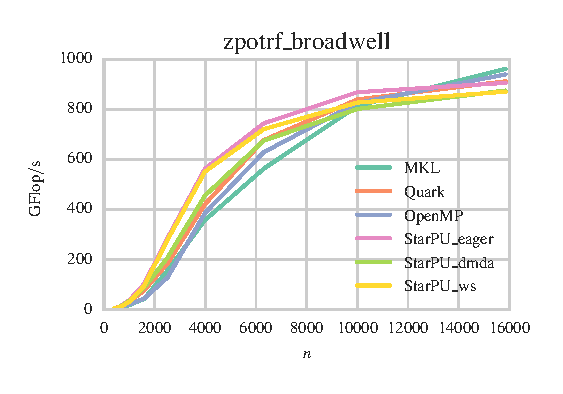
\includegraphics[scale=.85]{fig/kebnekaise_zpotrf_weak_scaling.eps}
  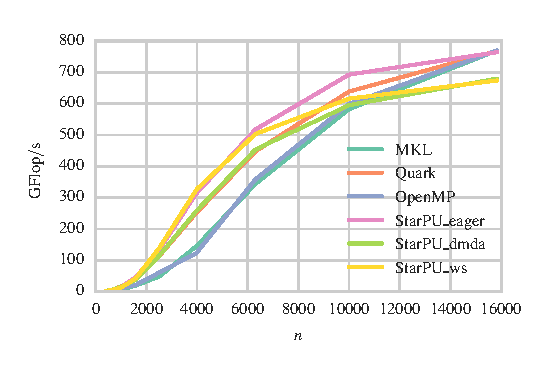
\includegraphics[scale=.85]{fig/kebnekaise_dpotrf_weak_scaling.eps}
  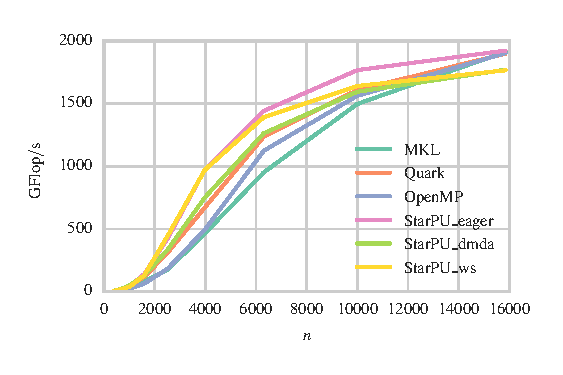
\includegraphics[scale=.85]{fig/kebnekaise_cpotrf_weak_scaling.eps}
  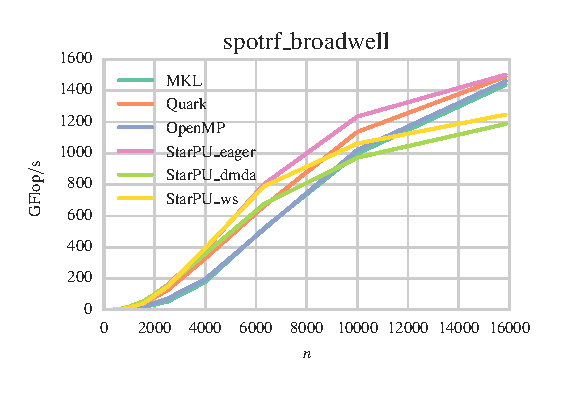
\includegraphics[scale=.85]{fig/kebnekaise_spotrf_weak_scaling.eps}
  \caption{Performance of Cholesky factorization on NUMA node.
    The top row has double complex precision on the left and double
    precision on the right.
    The bottom row has complex precision on the left and single
    precision on the right.}
  \label{fig.chol_numa}
\end{figure}

Figure~\ref{fig.chol_numa} gives the performance results
for computing a Cholesky factorization on the NUMA node
in each of the four standard precisions.
In all four precisions we see that StarPU with
the ``eager'' strategy gives the best performance over
essentially all matrix sizes.
This is closely followed by the ``ws'' strategy
and Quark.
In double complex precision the ``eager'' strategy
gives the best performance until matrices with
$n > 13000$ are considered,
after which MKL and OpenMP perform the factorization faster.

\begin{figure}[t]
  \centering
  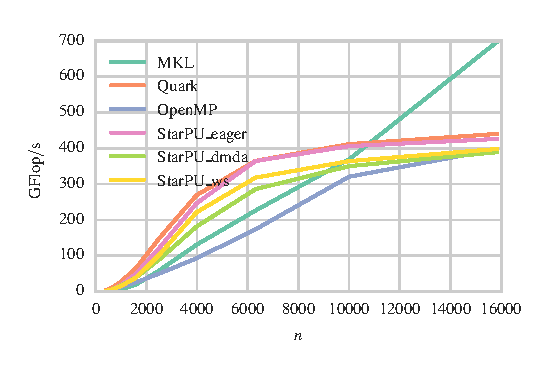
\includegraphics[scale=.85]{fig/knl_ram_zpotrf_weak_scaling.eps}
  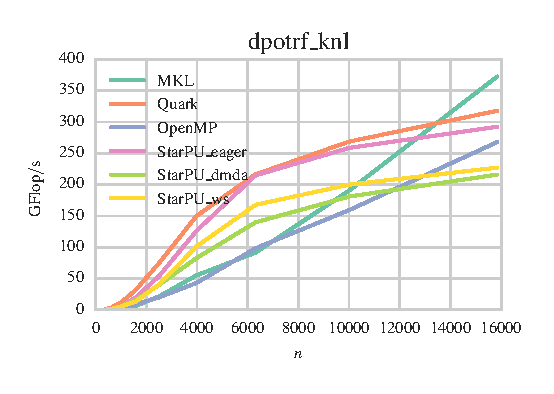
\includegraphics[scale=.85]{fig/knl_ram_dpotrf_weak_scaling.eps}
  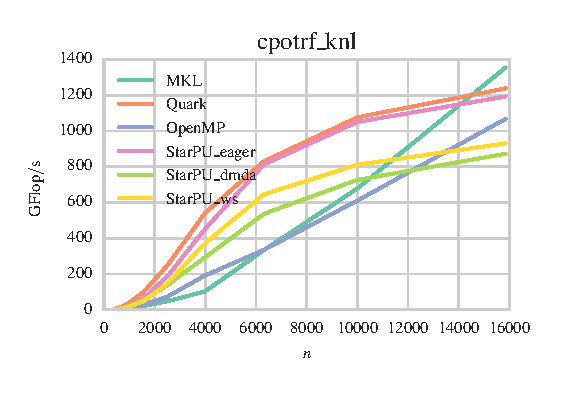
\includegraphics[scale=.85]{fig/knl_ram_cpotrf_weak_scaling.eps}
  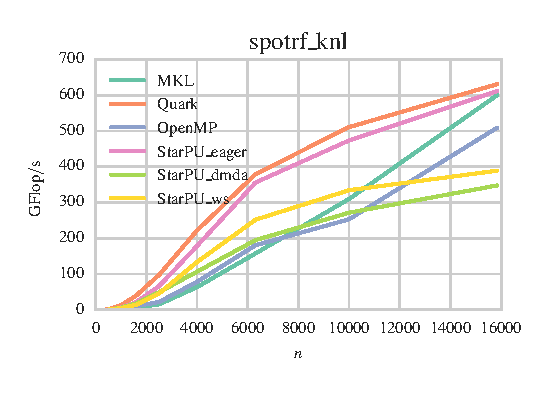
\includegraphics[scale=.85]{fig/knl_ram_spotrf_weak_scaling.eps}
  \caption{Performance of Cholesky factorization on the KNL.
    The top row has double complex precision on the left and double
    precision on the right.
    The bottom row has complex precision on the left and single
    precision on the right.}
  \label{fig.chol_knl_ram}
\end{figure}

In Figure~\ref{fig.chol_knl_ram} we perform the same experiment
on the KNL.
In all cases we see that Quark and StarPU with the ``eager''
scheduler are the best amongst the PLASMA implementations,
and the best overall until the largest test matrices are used.
OpenMP appears to be lagging behind the other implementations
in performance most of the time,
but does not suffer the same stagnation as Quark and StarPU.
Indeed MKL and OpenMP scale well as the matrix size increases:
the performance of the other PLASMA-based implementations
begins to stagnate whilst MKL and OpenMP keep increasing.
With further autotuning described in NLAFET deliverable D6.4
we will be able to increase the performance substantially.


%%%%%%%%%%%%%%%%%%%%%%%%%%%%%%
\section{$LU$ factorization}
\label{sec.lu}
%%%%%%%%%%%%%%%%%%%%%%%%%%%%%%
\begin{figure}[t]
  \centering
  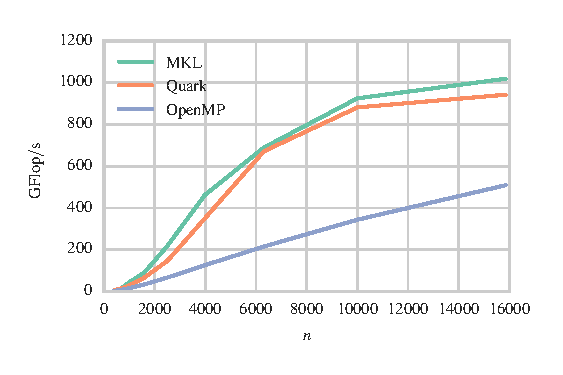
\includegraphics[scale=.85]{fig/kebnekaise_zgetrf_weak_scaling.eps}
  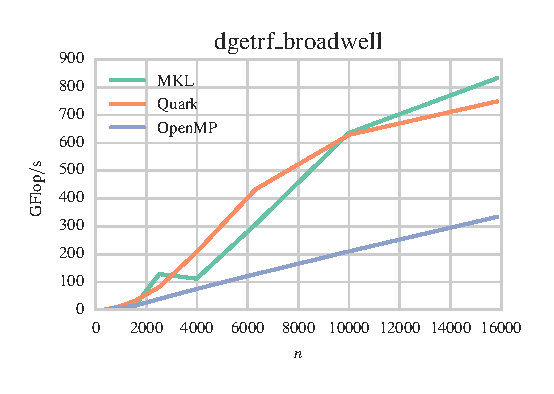
\includegraphics[scale=.85]{fig/kebnekaise_dgetrf_weak_scaling.eps}
  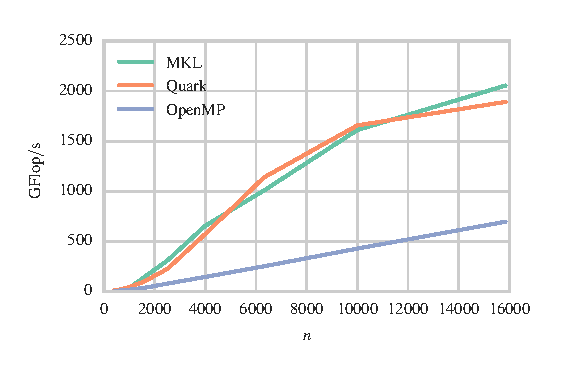
\includegraphics[scale=.85]{fig/kebnekaise_cgetrf_weak_scaling.eps}
  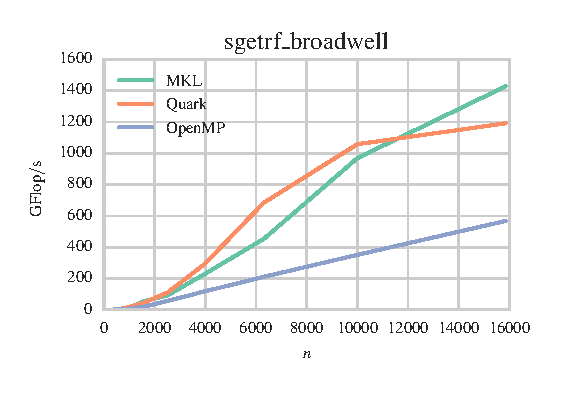
\includegraphics[scale=.85]{fig/kebnekaise_sgetrf_weak_scaling.eps}
  \caption{Performance of $LU$ factorization on NUMA node.
    The top row has double complex precision on the left and double
    precision on the right.
    The bottom row has complex precision on the left and single
    precision on the right.}
  \label{fig.lu_numa}
\end{figure}

Next we look at the $LU$ factorization.
The KStar source-to-source compiler was unable to convert
the OpenMP implementation into StarPU here,
due to the coding style utilized,
so the various StarPU versions do not appear in this section.

In Figure~\ref{fig.lu_numa} we plot the results from the NUMA node.
Here we see that MKL and Quark give
relatively similar performance,
though Quark is significantly slower for the larger matrices in our
experiments.
In all cases OpenMP lags behind all other implementations:
this is due to the way that task-dependencies have been expressed
in the new PLASMA implementation,
leading to less parallelism being expressed,
and should not be considered a deficiency of the runtime itself.
The PLASMA development team are currently exploring options
to rectify the situation which will be released imminently.

\begin{figure}[t]
  \centering
  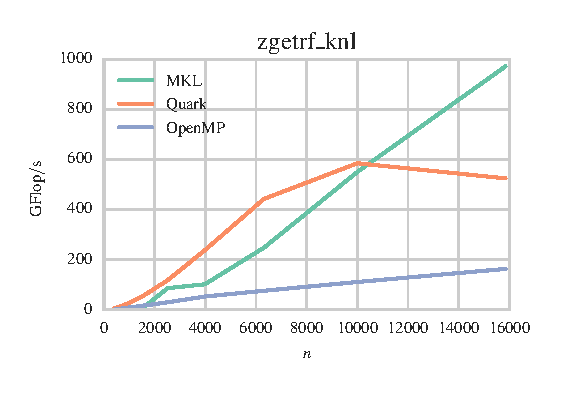
\includegraphics[scale=.85]{fig/knl_ram_zgetrf_weak_scaling.eps}
  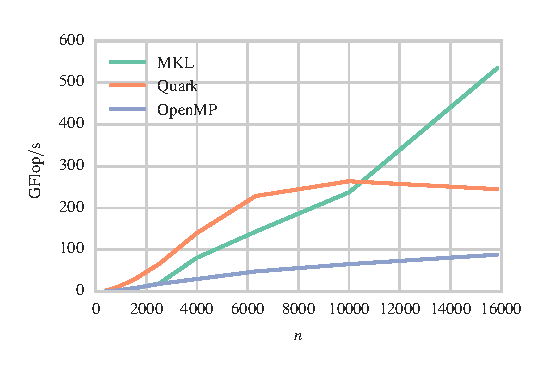
\includegraphics[scale=.85]{fig/knl_ram_dgetrf_weak_scaling.eps}
  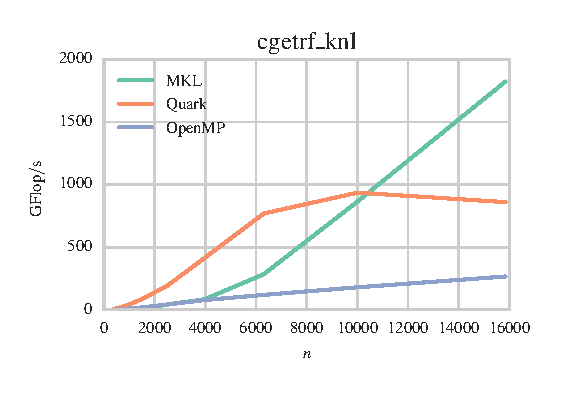
\includegraphics[scale=.85]{fig/knl_ram_cgetrf_weak_scaling.eps}
  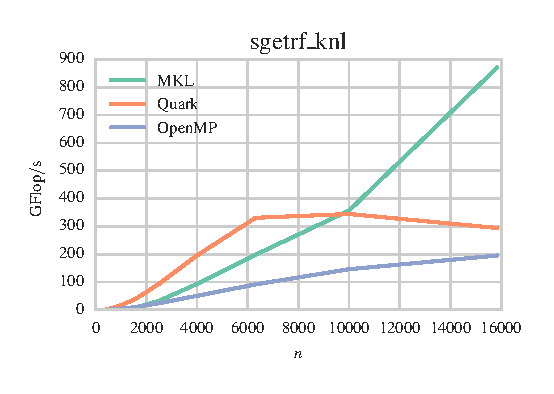
\includegraphics[scale=.85]{fig/knl_ram_sgetrf_weak_scaling.eps}
  \caption{Performance of $LU$ factorization on the KNL.
    The top row has double complex precision on the left and double
    precision on the right.
    The bottom row has complex precision on the left and single
    precision on the right.}
  \label{fig.lu_knl_ram}
\end{figure}

In Figure~\ref{fig.lu_knl_ram} we perform the same experiment
on the KNL system.
As before,
the MKL implementation scales well whilst
the performance of Quark stagnates and even decreases
slightly for very large matrices.
Meanwhile,
the lower level of parallelism expressed by the OpenMP
implementation leads to an enormous performance hit on the KNL:
the large number of cores need lots of parallelism
to be utilised efficiently.
When the OpenMP version is reimplemented we expect to see
performance similar to that of MKL.
One interesting feature of these plots is that for
the smaller matrices in our tests,
Quark is significantly faster than both MKL and LAPACK.

%%%%%%%%%%%%%%%%%%%%%%%%%%%%%%
\section{$QR$ factorization}
\label{sec.qr}
%%%%%%%%%%%%%%%%%%%%%%%%%%%%%%
\begin{figure}[t]
  \centering
  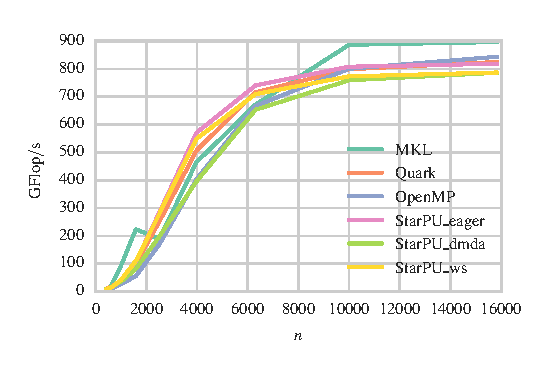
\includegraphics[scale=.85]{fig/kebnekaise_zgeqrf_weak_scaling.eps}
  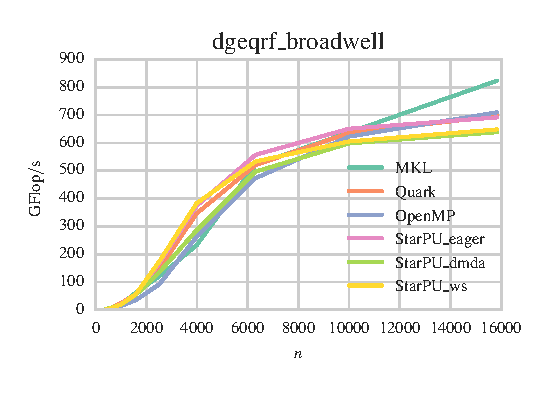
\includegraphics[scale=.85]{fig/kebnekaise_dgeqrf_weak_scaling.eps}
  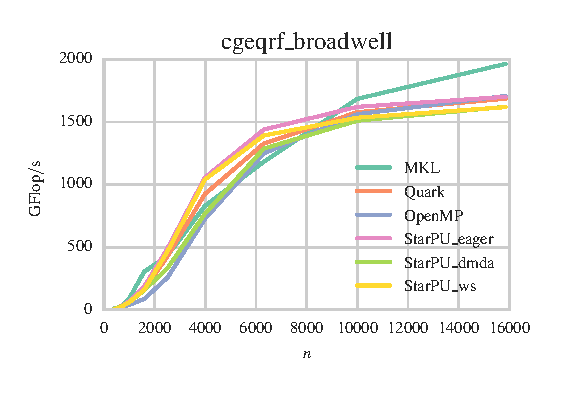
\includegraphics[scale=.85]{fig/kebnekaise_cgeqrf_weak_scaling.eps}
  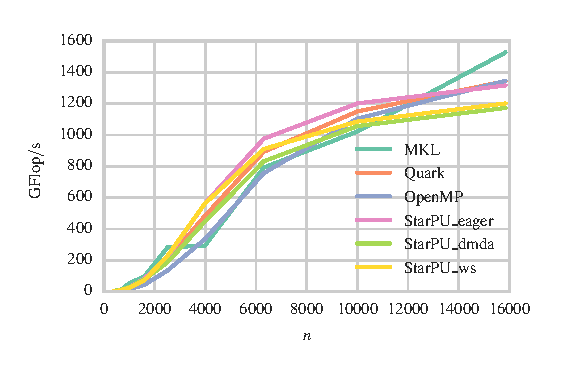
\includegraphics[scale=.85]{fig/kebnekaise_sgeqrf_weak_scaling.eps}
  \caption{Performance of $QR$ factorization on NUMA node.
    The top row has double complex precision on the left and double
    precision on the right.
    The bottom row has complex precision on the left and single
    precision on the right.}
  \label{fig.qr_numa}
\end{figure}

The third factorization we consider is $QR$.
The KStar source-to-source compiler was able to generate StarPU
code for this particular routine so all runtimes are present.

In Figure~\ref{fig.qr_numa} we have the performance of the different
implementations on the NUMA node for all four precisions.
For double and double complex precision on the top row,
we see that initially StarPU with the ``eager'' and ``ws'' strategies
perform best, closely followed by Quark.
However,
after matrices of size $8000$--$10000$ (depending upon the precision)
are considered,
MKL takes the lead whilst the
performance of the other runtimes begin to stagnate.
OpenMP is often the worst performer in these cases,
and also stagnates when larger matrices are used.
For complex and single precision the behaviour is rather similar,
though StarPU with the ``eager'' scheduler is competitive until
matrices of size larger than $10000$ are used.

\begin{figure}[t]
  \centering
  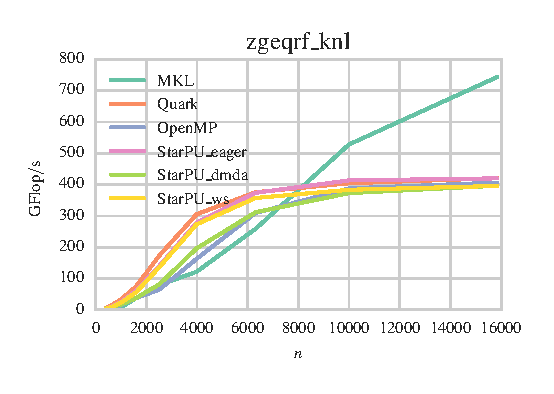
\includegraphics[scale=.85]{fig/knl_ram_zgeqrf_weak_scaling.eps}
  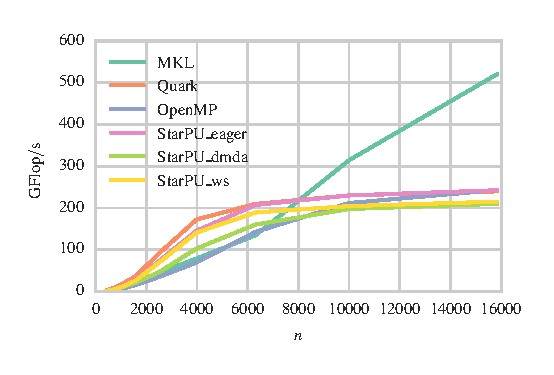
\includegraphics[scale=.85]{fig/knl_ram_dgeqrf_weak_scaling.eps}
  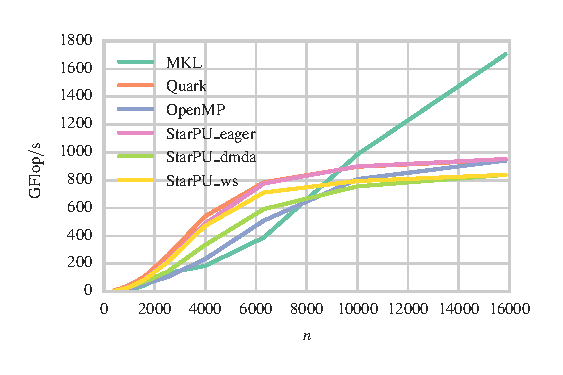
\includegraphics[scale=.85]{fig/knl_ram_cgeqrf_weak_scaling.eps}
  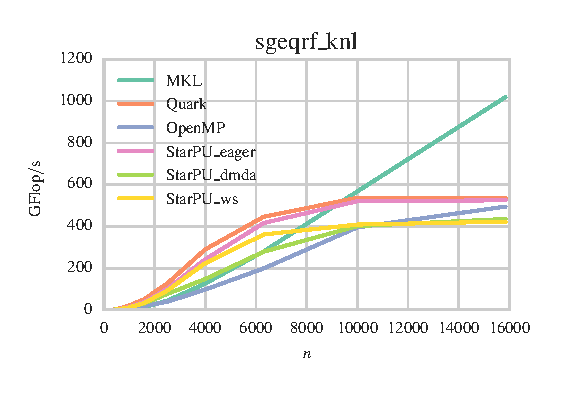
\includegraphics[scale=.85]{fig/knl_ram_sgeqrf_weak_scaling.eps}
  \caption{Performance of $QR$ factorization on the KNL.
    The top row has double complex precision on the left and double
    precision on the right.
    The bottom row has complex precision on the left and single
    precision on the right.}
  \label{fig.qr_knl_ram}
\end{figure}

We perform the same experiment on the KNL in
Figure~\ref{fig.qr_knl_ram}.
Here we see that all runtimes except for MKL stagnate very quickly
and give relatively poor performance by comparison.
These issues may well be resolved by utilising the
autotuning described in NLAFET deliverable D6.4.
Even though the performance leaves much to be desired,
we can see that StarPU with the ``eager'' strategy
and Quark perform significantly better than the
other PLASMA-based implementations.

%%%%%%%%%%%%%%%%%%%%%%%%%%%%%%
\section{Symmetric indefinite factorization}
\label{sec.ldlt}
%%%%%%%%%%%%%%%%%%%%%%%%%%%%%%
\begin{figure}[t]
  \centering
  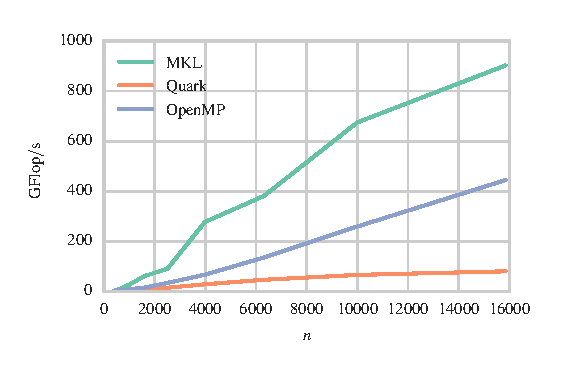
\includegraphics[scale=.85]{fig/kebnekaise_zhetrf_weak_scaling.eps}
  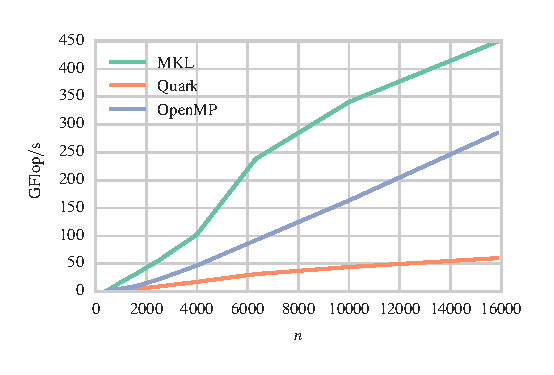
\includegraphics[scale=.85]{fig/kebnekaise_dsytrf_weak_scaling.eps}
  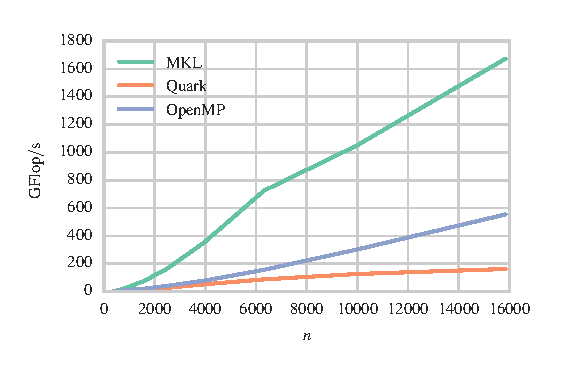
\includegraphics[scale=.85]{fig/kebnekaise_chetrf_weak_scaling.eps}
  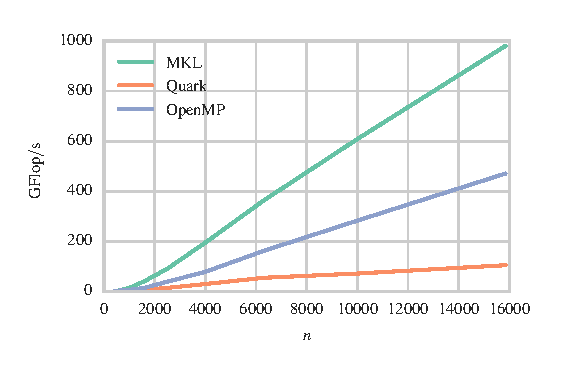
\includegraphics[scale=.85]{fig/kebnekaise_ssytrf_weak_scaling.eps}
  \caption{Performance of symmetric-indefinite factorization on NUMA node.
    The top row has double complex precision on the left and double
    precision on the right.
    The bottom row has complex precision on the left and single
    precision on the right.}
  \label{fig.ldlt_numa}
\end{figure}

Finally,
we look at the symmetric indefinite factorization.
Unfortunately, KStar could not generate a StarPU version of this
function so we can only compare OpenMP and Quark
MKL in this scenario.

The results obtained on the NUMA node are given in
Figure~\ref{fig.ldlt_numa}.
We see that clearly MKL is performing very well,
but OpenMP is significantly better than Quark.
Interestingly,
none of the implementations are stagnating when the larger matrices
are used.

\begin{figure}[t]
  \centering
  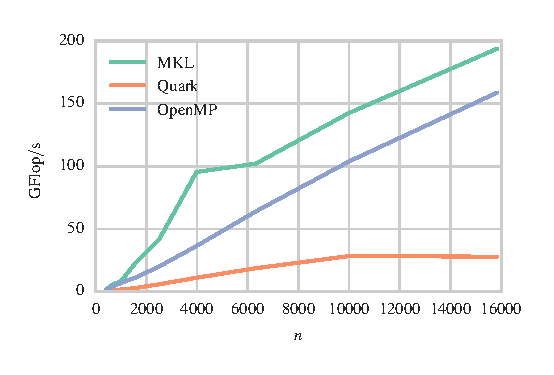
\includegraphics[scale=.85]{fig/knl_ram_zhetrf_weak_scaling.eps}
  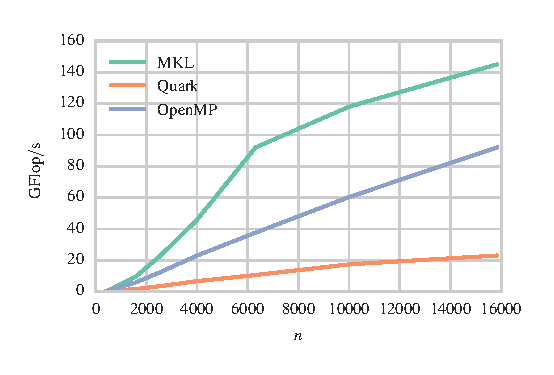
\includegraphics[scale=.85]{fig/knl_ram_dsytrf_weak_scaling.eps}
  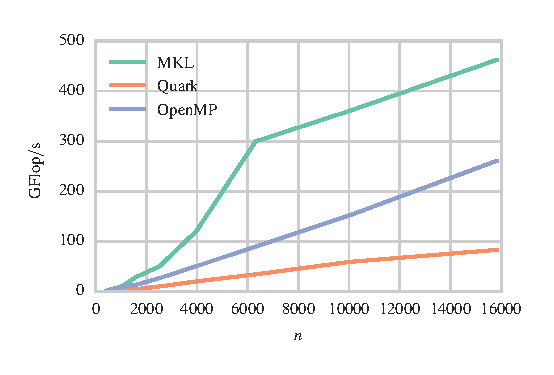
\includegraphics[scale=.85]{fig/knl_ram_chetrf_weak_scaling.eps}
  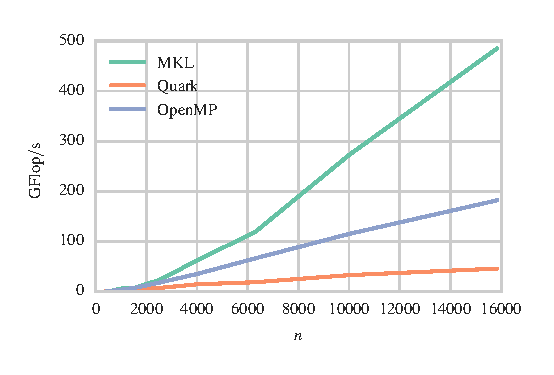
\includegraphics[scale=.85]{fig/knl_ram_ssytrf_weak_scaling.eps}
  \caption{Performance of symmetric-indefinite factorization on the KNL.
    The top row has double complex precision on the left and double
    precision on the right.
    The bottom row has complex precision on the left and single
    precision on the right.}
  \label{fig.ldlt_knl_ram}
\end{figure}

The corresponding results on the KNL are shown in
Figure~\ref{fig.ldlt_knl_ram}.
The behaviour is very similar to the previous experiment
although Quark appears to be stagnating in some of these experiments.

%%%%%%%%%%%%%%%%%%%%%%%%%%%%%%
\section{Conclusions}
\label{sec.conclusions}
%%%%%%%%%%%%%%%%%%%%%%%%%%%%%%

It is clear from our experiments that our current implementations in
Quark, OpenMP, and StarPU are not optimal.
In order to catch up with MKL for larger matrices a significant amount
of autotuning will need to be performed (see deliverable D6.4).
However,
the main goal of this report was to compare the various runtime
systems.

It is clear that,
when KStar was able to generate a StarPU version of our code,
that StarPU with either the ``eager'' or ``ws'' strategies
outperformed OpenMP and Quark.
Since StarPU also supports GPUs and distributed memory computation,
it is the clear winner in our runtime comparison.

In further work we hope to compare against PaRSEC,
once its source-to-source compiler is completed.
We would also like to recompare the PLASMA-based implementations
against LAPACK and MKL once the autotuning from deliverable D6.4
has been incorporated.

\bibliographystyle{plain}
\bibliography{strings,one-sided,svd_biblio}

%%%%%%%%%%%%%%%%%%%%%%%%%%%%%%%%%%%%%%%%%%%%%%%%%%%%%%%%%%%%
% END OF THE ACTUAL DELIVERABLE
%%%%%%%%%%%%%%%%%%%%%%%%%%%%%%%%%%%%%%%%%%%%%%%%%%%%%%%%%%%%

\end{document}
